\chapter{Implementação}\visiblelbl{chap:implementacao}

Neste capítulo, veremos os aspectos práticos do algoritmo, sua implementação, e 
detalhes computacionais. Vamos expandir a definição dos passos normal e
tangente,
detalhando os métodos internos para sua obtenção. Vamos considerar, ainda, o problema
no formato geral utilizado no repositório de testes CUTEr\cite{bib:cuter}.
Nossa implementação pode ser encontrada em \cite{bib:dcicpp}.

\section{Estruturas de Dados}\visiblelbl{sec:estruturas-de-dados}

Baseado no desempenho do algoritmo CDI para igualdades, decidimos utilizar a
fatoração de Cholesky para resolver os sistemas lineares de nosso método. Sendo
assim, procuramos uma implementação eficiente para usar como base de nosso
algoritmo. Encontramos a biblioteca CHOLMOD
\cite{bib:cholmod2,bib:cholmod3,bib:cholmod1,bib:cholmod4, bib:cholmod5},
escrita em C, que atendia aos nossos requisitos. Como trabalhamos em C++,
decidimos criar uma biblioteca chamada de \verb+base_matrices+
\cite{bib:base_matrices} para servir de embrulho para as estruturas do CHOLMOD.
As estruturas do CHOLMOD e seus respectivos embrulhos são
\begin{itemize}
 \item \verb+cholmod_common+ - \verb+base_common+ - Estrutura que guarda as
   parâmetros, estatísticas e o espaço de trabalho das variáveis.
 \item \verb+cholmod_sparse+ - \verb+base_sparse+ - Estrutura que guarda
   matrizes esparsas no formato de coluna comprimida.
 \item \verb+cholmod_factor+ - \verb+base_factor+ - Estrutura que guarda a
   fatoração de Cholesky de uma matriz esparsa.
 \item \verb+cholmod_dense+ - \verb+base_dense+ - Estrutura que guarda matrizes
   ou vetores densos.
 \item \verb+cholmod_triplet+ - \verb+base_triplet+ - Estrutura que guarda
   matrizes esparsas no formato de triplas. É usada para receber facilmente os
   dados, e passá-los para o formato de coluna comprimida.
\end{itemize}

Também definimos tipos básicos de variáveis, considerando a possibilidade
de expansão do algoritmo além dos tipos básicos de \verb-C/C++-, e considerando
a compatibilidade com Fortran e CUTEr.
Atualmente, os tipos que temos são
\begin{itemize}
  \item \verb+Real+ - Corresponde ao tipo \verb+double+;
  \item \verb+Int+  - Corresponde ao tipo \verb+int+;
  \item \verb+Bool+ - Corresponde ao tipo \verb+int+.
\end{itemize}
Os tipos foram implementados de modo a permitir mudanças nas definições. Dessa
maneira, o usuário que quiser utilizar alguma precisão diferente precisará
mudar pouca coisa antes da compilação.

\section{Interface CUTEr}

Nosso algoritmo, intitulado \verb+DCICPP+ (do inglês, {\it Dynamic Control of
Infeasibility - C Plus Plus}), trabalha com uma classe de interface,
que recebe todas as informações necessárias para resolver o problema, como a
função objetivo, as derivadas, e as restrições.
Como decidimos utilizar as funções definidas pelo CUTEr como modelo para nossas
funções, é esperado que o desempenho de um problema do CUTEr e de um
problema feito ``à mão'' sejam equivalentes, em relação às chamadas de função.
Obviamente, o custo de se calcular a função varia pois, em uma maneira, o
usuário define-a explicitamente e, em outra, o CUTEr é responsável por retornar
o valor.

O problema é recebido no formato utilizado pelo CUTEr, que é dado por
%\ref{prob:geral_cuter}
\begin{equation} \visiblelbl{prob:geral_cuter_local}
\begin{array}{rrrcll}
\min       & f(x) \\
\mbox{s.a} &     &      & c_E(x) &   =  & 0, \\
           & c_L & \leq & c_I(x) & \leq & c_U, \\
           & b_L & \leq &     x  & \leq & b_U.
\end{array}
\end{equation}
Para resolver um problema, é preciso fornecer uma quantidade mínima de
informações, tais como um ponto inicial $x^0$ e os limitantes para as variáveis,
$b_L$ e $b_U$. 
Para indicar que o limitante superior não existe, definimos $b_{U_i} = 10^{20}$,
e para indicar que o limitante inferior não existe, definimos $b_{L_i} =
-10^{20}$. Além disso, o usuário precisa definir as funções computacionais que
calculam os valores das funções matemáticas e suas derivadas, e, se o problema
for irrestrito, alguns outros vetores com informações pertinentes.

Vamos apresentar agora as funções que o usuário precisa definir para executar o
programa. Como alternativa, ele pode criar um arquivo \verb+SIF+ para o CUTEr,
contendo as informações do problema, e resolver o problema usando o DCICPP para
o CUTEr, apesar dessa estratégia ser, em geral, mais trabalhosa.
É importante notar que, por compatibilidade com o CUTEr, que está em Fortran,
todos os argumentos de função são ponteiros. Então, mesmo valores triviais, como
o número de variáveis, são passados como ponteiros.

Para problemas irrestritos, é necessário definir as seguintes funções:
\begin{itemize}
  \item \verb+void UFN(Int *n, Real *x, Real *f)+ \\
    Calcula o valor da função objetivo \verb+*f+ no ponto \verb+x+, que tem
    dimensão \verb+*n+.
  \item \verb+void UOFG(Int *n, Real *x, Real *f, Real *g, Bool *grad)+ \\
    Calcula o valor da função objetivo \verb+*f+, no ponto \verb+x+, que tem
    dimensão \verb+*n+. Se \verb+*grad+ for $1$, então também retorna o
    gradiente da função objetivo \verb+g+.
  \item \verb+void UPROD(Int *n, Bool *getder, Real *x, Real *p, Real *q)+ \\
    Calcula o produto da Hessiana no ponto \verb+x+ por \verb+p+ e retorna o
    valor em \verb+q+, isto é, retorna $q = \nabla^2 f(x)p$. Os vetores
    \verb+x+, \verb+p+ e \verb+q+ têm dimensão \verb+*n+. A variável
    \verb+*getder+ é sempre igual a $0$ em nossa implementação.
\end{itemize}
Para problemas restritos, o usuário precisa definir as seguintes funções:
\begin{itemize}
  \item \verb+void CFN(Int *n, Int *m, Real *x, Real *f, Int *lc, Real *c)+ \\
    Calcula o valor da função objetivo \verb+*f+ e o vetor de restrições
    \verb+c+ no ponto \verb+x+. A dimensão de \verb+x+ é \verb+*n+ e a dimensão
    de \verb+c+ é \verb+*m+. O Valor \verb+*lc+ é a dimensão real de \verb+c+,
    que em nosso caso é sempre igual a \verb+*m+.
  \item \verb+void COFG(Int *n, Real *x, Real *f, Real *g, Bool *grad)+ \\
    Calcula o valor da função objetivo \verb+*f+ no ponto \verb+x+, que tem
    dimensão \verb+*n+. Se \verb+*grad+ for $1$, então também retorna o
    gradiente da função objetivo \verb+g+.
  \item 
    \verb+void CPROD(Int *n, Int *m, Bool *getder, Real *x, Int *ly,+ \\
    \verb+           Real *y, Real *p, Real *q)+ \\
    Calcula o produto da Hessiana do Lagrangeano no ponto \verb+x+, com
    multiplicadores \verb+y+, pelo vetor \verb+p+, retornando o vetor \verb+q+,
    isto é, retornando $q = \nabla_{xx}^2\mathcal{L}(x,y)p$. \verb+x+, \verb+p+
    e \verb+q+ têm dimensão \verb+*n+, e \verb+y+ tem dimensão \verb+*m+.  o
    valor \verb+*getder+ é sempre $0$. O valor \verb+*ly+ é a dimensão real de
    \verb+y+, que em nosso caso é sempre igual a \verb+*m+.
  \item 
    \verb+void CCFSG(Int *n, Int *m, Real *x, Int *lc, Real *c,+\\
    \verb+           Int *nnzJ, Int *amax, Real *J, Int *indvar,+\\
    \verb+           Int *indfun, Bool *grad)+\\
    Calcula o valor das restrições \verb+c+ e, se \verb+*grad+ for igual a 1,
    também a Jacobiana das restrições no ponto \verb+x+, guardando-a na forma de
    triplas, de modo que os valores $J_{ij}$ são guardados em \verb+J+, os índices
    das linhas são guardados em \verb+indfun+ e os índices das colunas são
    guardados em \verb+indvar+. Apenas os valores não nulos são retornados. 
    A dimensão de \verb+x+ é \verb+*n+. A dimensão de \verb+c+ é \verb+*m+.
    O vetor \verb+*lc+ é a dimensão real de \verb+c+, que em nosso caso é sempre
    igual a \verb+*m+. O valor \verb+*nnzJ+ é o número de elementos não nulos da
    Jacobiana, e \verb+*amax+ é a dimensão declarada de \verb+J+, \verb+indvar+
    e \verb+indfun+, que tem que ser maior ou igual a \verb+*nnzJ+.
\end{itemize}
Se o problema é restrito, além dessas funções o usuário também precisa fornecer
um vetor binário \verb+equatn+, de dimensão $m$, indicando quais restrições são
de igualdade e quais são de desigualdade. Também é necessário fornecer os
limitantes $c_L$ e $c_U$ das restrições, de modo que, se a restrição $i$ for de
igualdade, então $c_{L_i} = c_{U_i} = 0$, e se for de desigualdade, então
$c_{L_i} < c_{U_i}$.
Finalmente, também é necessário fornecer \verb+amax+, a quantidade máxima de
elementos não nulos na Jacobiana.
Se a restrição for ilimitada superiormente, defina $c_{U_i}
= 10^{20}$, e se for ilimitada inferiormente, defina $c_{L_i} = -10^{20}$.
Opcionalmente, o usuário pode passar o vetor \verb+linear+ indicando quais
restrições são lineares. No entanto, ainda não estamos usando essa propriedade em
todo o seu potencial.

O Apêndice \ref{ap:interface_cuter} mostra o arquivo de interface do CUTEr, e dois
arquivos de exemplo para criação de problemas.

\section{Generalização}\visiblelbl{sec:generalizacao}

Os teoremas apresentados nas seções anteriores foram desenvolvidos em torno do
problema \eqref{prob:geral}, que é o problema geral em um formato mais simples.
No entanto, a implementação do método segue o formato utilizado pela biblioteca
de testes CUTEr \cite{bib:cuter}, mostrado em \eqref{prob:geral_cuter_local}.
Naturalmente, é possível converter o problema acima para o formato geral
\eqref{prob:geral}, definindo 
$$\tilde{c}_I(x) =
\left[
\begin{array}{c}
c_I(x) - c_L \\
c_U - c_I(x) \\
x - b_L \\
b_U - x
\end{array}\right],
$$
de modo a obter o problema
\begin{equation}\nonumber
\begin{array}{rrcl}
 \min      & f(x) \\
\mbox{s.a} & c_E(x) & = & 0, \\
& \tilde{c}_I(x) & \geq & 0.
\end{array}
\end{equation}
No entanto, para trabalhar com esse problema, teríamos que lidar com a Jacobiana
de $\tilde{c}_I$, cuja fatoração e armazenamento são caros.
Decidimos, então, trabalhar com o formato do CUTEr e expandir o método para esse
caso.

Nossa estratégia começa transformando o problema \eqref{prob:geral_cuter_local}
num problema de igualdade com limitantes nas variáveis. Para isso, introduzimos
uma variável $s\in\Rn{m_I}$, obtendo
\begin{equation}\nonumber
\begin{array}{rrrcll}
\min       & f(x) \\
\mbox{s.a} & & & c_E(x) & = & 0, \\
           & & & c_I(x) - s & = & 0, \\
           & b_L & \leq & x & \leq & b_U, \\
           & c_L & \leq & s & \leq & c_U.
\end{array}
\end{equation}
Agora, definimos a variável
$$z = \vetor{x}{s},$$
a função
$$h(z) = \vetor{c_E(x)}{c_I(x) - s},$$
e os vetores
$$l = \vetor{b_L}{c_L} \qquad u = \vetor{b_U}{c_U},$$
para obter o problema
\begin{equation}\nonumber
\begin{array}{rl}
\min       & f(x) \\
\mbox{s.a} & h(z) = 0, \\
           & l \leq z \leq u.
\end{array}
\end{equation}
Lembramos que a variável $\ell_i$ pode valer $-\infty$, e $u_i$ pode valer
$\infty$, indicando que a componente $i$ da variável $z$ não tem limitante
inferior ou superior, respectivamente. Note que podemos ter uma variável sem
limitante algum.

Finalmente, vamos transformar esse problema no problema de pontos interiores,
\begin{equation}\visiblelbl{prob:geral_pto_int}
 \begin{array}{rl}
  \min & \varphi(z,\mu) = f(x) + \mu \beta(z)\\
  \mbox{s.a} & h(z) = 0,
 \end{array}
\end{equation}
onde $\beta$ é uma função que se aproxima do infinito quando alguma componente
de $z$ se aproxima de seu limitante. Nossa ideia inicial foi fazer
$$\beta(z) = -\sum_{i : \ell_i>-\infty}\log(z_i - \ell_i) -
\sum_{i:u_i<\infty}\log(u_i-z_i).$$
Nesse caso, nossa matriz de escalamento seria definida como
$\Lambda(z) = (\Lambda_1(z),\dots,\Lambda_N(z))$, onde
\begin{equation}
\Lambda_i(z) = \left\{
 \begin{array}{ll}
  1,                      & \mbox{se } \ell_i = -\infty \mbox{ e } u_i = \infty, \\
  (z_i - \ell_i),            & \mbox{se } \ell_i > -\infty \mbox{ e } u_i =
   \infty, \\
  (u_i - z_i),            & \mbox{se } \ell_i = -\infty \mbox{ e } u_i < \infty, \\
  (z_i - \ell_i)(u_i - z_i), & \mbox{se } \ell_i > -\infty \mbox{ e } u_i <
   \infty.
 \end{array}\right.
\end{equation}
Lembramos que esse escalamento provém da necessidade de melhorar a estabilidade
das derivadas do problema. Assim, dada uma componente $i$ de $z$ que tenha
limitante inferior e superior, a componente $i$ de $\Lambda(z) \nabla \beta(z)$
será
\begin{eqnarray*}
 \Lambda_i(z) \frac{\partial \beta(z)}{\partial z_i}(z) & = &
- (z_i - \ell_i)(u_i - z_i) \bigg[\frac{1}{z_i - \ell_i} - \frac{1}{u_i -
    \ell_i}\bigg], \\
& = & - [u_i - z_i - (z_i - \ell_i)], \\
& = & 2z_i - \ell_i - u_i.
\end{eqnarray*}
Podemos ver que essa componente pode gerar dificuldades computacionais caso
$z_i$ fique muito grande. Desse modo, nossa estratégia inicial não é
satisfatória.

Decidimos, então, testar uma barreira $\beta$ alternativa. Nossa escolha foi
$$\beta(z) = -\sum_{i=1}^n\beta_i(z),$$
onde
\begin{equation}
 \beta_i(z) = \left\{
\begin{array}{ll}
 0,              &  \mbox{se } \ell_i = -\infty \mbox{ e } u_i = \infty, \\
 \log(z_i - \ell_i),&  \mbox{se } \ell_i > -\infty \mbox{ e } u_i = \infty, \\
 \log(u_i - z_i),&  \mbox{se } \ell_i = -\infty \mbox{ e } u_i < \infty, \\
 \log(z_i - \ell_i),&  \mbox{se } \ell_i > -\infty \mbox{ e } u_i < \infty \mbox{ e } 
z_i < (u_i + \ell_i)/2, \\
 \log(u_i - z_i),&  \mbox{se } \ell_i > -\infty \mbox{ e } u_i < \infty \mbox{ e } 
z_i \geq (u_i + \ell_i)/2.
\end{array}
\right.
\end{equation}
Essa escolha difere quando uma variável é limitada superior e inferiormente.
Nesse caso, escolhemos penalizar de acordo com a proximidade ao limitante.
A matriz de escalamento correspondente a essa barreira é
\begin{equation}
 \Lambda_i(z) = \left\{
\begin{array}{ll}
 0,         & \mbox{se } \ell_i = -\infty \mbox{ e } u_i = \infty, \\
 z_i - \ell_i, & \mbox{se } \ell_i > -\infty \mbox{ e } u_i = \infty, \\
 u_i - z_i, & \mbox{se } \ell_i = -\infty \mbox{ e } u_i < \infty, \\
 z_i - \ell_i, & \mbox{se } \ell_i > -\infty \mbox{ e } u_i < \infty \mbox{ e } 
z_i < (u_i + \ell_i)/2, \\
 u_i - z_i, & \mbox{se } \ell_i > -\infty \mbox{ e } u_i < \infty \mbox{ e } 
z_i \geq (u_i + \ell_i)/2.
\end{array}
\right.
\end{equation}
Com essa nova barreira, agora temos a componente $i$ do produto $\Lambda(z)\nabla \beta(z)$ 
constante:
\begin{eqnarray*}
\Lambda_i\frac{\partial \beta(z)}{\partial z_i} = 
\left\{
\begin{array}{ll}
 -1, & z_i < (u_i + \ell_i)/2, \\
  1, & z_i > (u_i + \ell_i)/2.
\end{array}\right.
\end{eqnarray*}
Note que as funções $\beta_i$ e $\Lambda_i$ são contínuas, porém não são
diferenciáveis para $z_i = (u_i + \ell_i)/2$ se os limitantes forem finitos. 
Uma alternativa para contornar esse problema é suavizar $\Lambda_i$.
Nesse caso, quando $\ell_i > -\infty$ e $u_i < \infty$, definimos $\Lambda_i$
como
\begin{equation*}
  \Lambda_i(z_i) = \left\{
  \begin{array}{ll}
    \dfrac{u_i-\ell_i}{2} -\modulo{ z_i - \dfrac{\ell_i+u_i}{2} }, &
      \qquad \mbox{se } \modulo{z_i-\dfrac{\ell_i+u_i}{2}} > \sigma_i \\
    \dfrac{u_i-\ell_i}{2}-\dfrac{\sigma_i}{2} -
    \dfrac{1}{2\sigma_i}\bigg(z - \dfrac{l+u}{2}\bigg)^2, &
      \qquad \mbox{caso contrário},
  \end{array}
  \right.
\end{equation*}
onde $\sigma_i > 0, i = 1,\dots,n+m_I$ são constantes, preferencialmente 
pequenas, que satisfazem $0 < \sigma_i < (u_i-\ell_i)/2$. A Figura \ref{fig:lambda}
mostra o formato de função $\Lambda_i(z_i)$.
\begin{figure}[H]
\centering
\begin{tikzpicture}
  \draw[->] (-1.1,0) -- (4.1,0);
  % l = -0.5, u = 3.5
  % u - l = 4, u + l = 3
  \draw[domain=-0.5:1.25] plot (\x,{2 - abs(\x-1.5)});
  \draw[domain=1.75:3.5] plot (\x,{2 - abs(\x-1.5)});
  \draw[domain=1.25:1.75] plot (\x,{2-0.25/2-0.5*(\x-1.5)*(\x-1.5)/0.25});
  \draw (-0.5,0.1) -- (-0.5,-0.1)node[below] {$\ell$};
  \draw ( 3.5,0.1) -- ( 3.5,-0.1)node[below] {$u$};
  \draw ( 1.5,0.1) -- ( 1.5,-0.1)node[below] {$\dfrac{\ell+u}{2}$};
  \draw[gray] (1.5,0) -- (1.5,{2-0.125});
  \draw[gray] (1.25,0) -- (1.25,1.75);
  \draw[gray] (1.75,0) -- (1.75,1.75);
  \draw[<->] (1.25,0.1) -- (1.5,0.1)node[above,midway] {$\sigma$};
  \draw[<->] (1.75,0.1) -- (1.5,0.1)node[above,midway] {$\sigma$};
\end{tikzpicture}
\caption{Ilustração da escolha de $\Lambda_i(z_i)$.}
\label{fig:lambda}
\end{figure}
Na nossa implementação, escolhemos $\sigma_i = 0.01(u_i-\ell_i)/2$ e definimos
$\beta$ como
$$ \beta(z) = \sum_{i=1}^{n+m_I}\beta_i(z_i) = \sum_{i=1}^{n+m_I}\ln(\Lambda_i(z)). $$
Com essa definição, temos
$$ \beta_i'(z_i) = \frac{\Lambda_i'(z_i)}{\Lambda_i(z_i)}, $$
e, para $\ell_i > -\infty$ e $u_i < \infty$, temos
\begin{equation*}
  \beta_i(z_i)\Lambda_i(z_i) = \Lambda_i'(z_i) = \left\{
  \begin{array}{ll}
    1, & z_i < \dfrac{\ell_i+u_i}{2} - \sigma_i, \\
    -\dfrac{1}{\sigma_i}\bigg(z - \dfrac{\ell_i+u_i}{2}\bigg), &
      \bigg|z_i-\dfrac{\ell_i+u_i}{2}\bigg| \leq \sigma_i, \\
    -1, & z_i > \dfrac{\ell_i+u_i}{2} + \sigma_i.
  \end{array}\right.
\end{equation*}

\section{Passo Normal e Atualização de $\rho$}

A iteração $k$ do algoritmo começa com o passo normal,
que consiste em encontrar um ponto $\zc{k}$ e atualizar o cilindro
$\rho^k$ de modo que $\norma{\zc{k}} \leq \rho^k$.
Durante o passo normal, também atualizamos $\mu^k$ e $\lambda^k$. 
Esse passo é obtido por uma sequência de passos internos que resolvem
aproximadamente o problema
\begin{equation}\visiblelbl{prob:normal_geral}
  \begin{array}{rc}
  \min & \displaystyle\meio\norma{h(z)}^2 \\
       & l \leq z \leq u.
  \end{array}
\end{equation}
Inicialmente, o cilindro tem raio $\rho^{k-1}$. 
Quando conseguirmos um ponto dentro desse cilindro, atualizamos seu raio, e
atualizamos os multiplicadores.  Se o ponto continuar dentro do cilindro, o
definimos como o ponto $\zc{k}$. Caso contrário, repetimos o procedimento.  O
algoritmo \ref{alg:passo_normal} explica o procedimento.
\begin{algorithm}[H]
\caption{Iteração $k$ do Passo Normal}
\label{alg:passo_normal}
\begin{algorithmic}[1]
  \State Dados $\phi_1 \in [10^{-4},1]$, $\rho = \rho^{k-1}$, $z_c = z^{k-1}$, e $\lambda =
 \lambda^{k-1}$
\State Atualize $\barra{A}$ e $\barra{J}$.\label{alg:jacob_update}
\State Faça $\Delta_N = \Delta_0$
\While{$\norma{h(z_c)} > \rho$}
  \State Calcule $z_c$ tal que $h(z_c)\leq\rho$ pelo {\bf passo normal interno}
    \visiblelbl{alg:passo_normal_interno}
\algstore{alg:passo.normal}
\end{algorithmic}
\end{algorithm}
\begin{algorithm}[H]
\caption*{Continuação do Algoritmo \ref{alg:passo_normal}}
\begin{algorithmic}
  \algrestore{alg:passo.normal}
  \State Atualize $\lambda$\label{alg:lambda_update}
  \State Calcule $g_p = g(z_c,\mu) + \barra{A}^T\lambda$
  \State Calcule $n_p = \norma{g_p}/(\norma{g(z_c,\mu)} + 1)$
  \If{$\rho > 2\rhomax n_p$}
    \State $\rho = \min\{\phi_1n_p, \max\{10^{-4}n_p, 0.75\}\}\rhomax$
  \Else
    \State $\rho = \max\{\rho, \min\{\phi_1\rhomax n_p, \max\{10^{-4}\rhomax n_p, 0.75\rhomax\}
\}\}$
  \EndIf
  \State $\rho = \max\{\rho, \varepsilon_h\}$
  \State $\mbox{gap} = \norma{\mu\nabla \beta_s(z) - \Lambda_s\lambda_I} + \norma{g_p} + 
\norma{h(z_c)}$
  \State $\mu = \min\{\mu, 100\rho, 100\rho^2, \mbox{gap}, 100\norma{h(z^{k-1})} \}$
\label{alg:gap}
\EndWhile
\State Faça $\zc{k} = z_c$, $\rho^k = \rho$ e $\lambda^k = \lambda$.
\end{algorithmic}
\end{algorithm}
No passo \ref{alg:jacob_update}, atualizamos as matrizes $\barra{A}$ e
$\barra{J}$. Como sugerido na Seção \ref{sec:conv-local}, essas matrizes são tais que
$$\norma{\barra{A} - A(z_c)} = \bigo(\norma{\gpk{k}}) \qquad \mbox{e} \qquad
\norma{\barra{J} - \nabla h(z_c)} = \bigo(\norma{\gpk{k}}).$$
Nossa estratégia atual consiste em tomar simplesmente $\barra{A} = A(z_c)$ e 
$\barra{J} = \nabla h(z_c)$.

\subsection{O Passo Normal Interno}\visiblelbl{sec:normal.step.internal}

No passo \ref{alg:passo_normal_interno} do algoritmo \ref{alg:passo_normal},
calculamos o passo normal interno do método.
O objetivo do passo interno é, dado $\rho > 0$, obter um ponto dentro do
cilindro de raio $\rho$. 
Segundo a Hipótese \ref{hip:local.normal.step}, esperamos que,
assintoticamente, os passos tenham a forma
$$\delta_N^+ = -\barra{J}^T(\barra{J}\barra{J}^T)^{-1}h(z_c),$$
chamada de forma de Gauss-Newton.
Vamos utilizar uma modificação do Método de Dogleg, na linha de
\cite{bib:francisco,bib:porcelli}, para obter o ponto acima, e vamos utilizar a
teoria de convergência destes métodos para mostrar que o método deve encontrar o
ponto dentro do cilindro, e também que, assintoticamente, o passo de Gauss-Newton
é utilizado.

A estratégia consiste em escolher um passo que seja combinação convexa
da projeção dos passos de Cauchy 
$d_C = -\alpha_C \barra{J}^Th(z_c)$ 
e de Gauss-Newton
$d_N = -\barra{J}(\barra{J}\barra{J}^T)^{-1}h(z_c)$
no interior da caixa definida pelos limitantes 
\begin{eqnarray*}
  \ell_{N_i} & = & \left\{
\begin{array}{ll}
 -\Delta_N, & \mbox{se } \ell_i = -\infty, \\
 \max\{-\Delta_N, (\ell_i - z_{c_i})(1 - \epsmu)\} & \mbox{caso contrário},
\end{array}
\right. \\
u_{N_i} & = & \left\{
\begin{array}{ll}
 \Delta_N, & \mbox{se } u_i = \infty \\
 \min\{\Delta_N, (u_i - z_{c_i})(1 - \epsmu)\} & \mbox{caso contrário},
\end{array}
\right.
\end{eqnarray*}
Note que esses limitantes provêm de
\begin{equation}
  l + \epsmu(z_c-l) \leq z_c + d \leq u - \epsmu(u-z_c),
\end{equation}
que é a generalização da condição de fração-para-a-fronteira \eqref{eq:slim}.
O Algoritmo \ref{alg:passo_porcelli} exibe os procedimentos.
\begin{algorithm}[H]
\caption{Passo Normal Interno}\label{alg:passo_porcelli}
\begin{algorithmic}[1]
\State Dados $\beta_1, \beta_2, \beta_3, \theta\in(0,1)$, $z_N^0 = z_c, \rho$
\While{ $\norma{h(\znj)} > \rho$ }
  \State Defina $m(\delta) = \meio\norma{\barra{J}\delta + h(\znj)}^2$
  \State Calcule $v = \nabla m(0) = \barra{J}^Th(\znj)$.
  \State Defina a matriz $D = \mbox{diag}(w_1,\dots,w_N)$, onde
\begin{equation}
  w_i = \left\{
  \begin{array}{ll}
    (u_{N_i} - z_i)^{-1/2}, & \mbox{se } v_i < 0 \mbox{ e } u_{N_i} <
    \infty, \\
    (z_i - \ell_{N_i})^{-1/2}, & \mbox{se } v_i > 0 \mbox{ e } \ell_{N_i} >
    -\infty, \\
  1, & \mbox{caso contrário}.
  \end{array} \right.
\end{equation}
  \State $d = -D^{-2}v$
  \State $\gamma(\delta) = \arg\max\{t \geq 0: \ell_{N_i}\leq t\delta \leq
    u_{N_i}\}$
  \State Defina
\begin{equation}
   P(\delta) = \left\{
    \begin{array}{ll}
    \delta, & \mbox{se } \gamma(\delta) > 1 \\
    \max\{\theta, 1 - \norma{\delta}\}\gamma(\delta)\delta, & \mbox{caso
      contrário}
  \end{array}\right.
\end{equation}
  \algstore{alg:normal.interno}
\end{algorithmic}
\end{algorithm}
\begin{algorithm}[H]
\caption*{Continuação do Algoritmo \ref{alg:passo_porcelli}}
\begin{algorithmic}
  \algrestore{alg:normal.interno}
  \State Calcule
\begin{equation}
  \alpha_{cp} = \arg\min_{\alpha}\bigg\{ \meio \norma{\alpha\barra{J} +
    h(\znj)}^2 : \alpha \norma{Dd} \leq \Delta_N\bigg\}
\end{equation}
  \State Defina $d_{cp} = P(\alpha_{cp}d)$.
  \State Defina
    $$\rho_C(\delta) = \frac{m(0) - m(\delta)}{m(0) - m(d_{cp})}$$
  \State Calcule $\barra{d}_N$, solução aproximada de $\min\{m(\delta) : 
    \norma{D\delta} \leq \Delta_N\}.$\label{alg:sol_aprox_newton}
  \State Defina $d_N = P(\barra{d}_N)$.
  \State Faça $t = 1$
  \While{$\rho_C(t d_N + (1 - t) d_{cp}) \geq \beta_1$}
    \State $t = 0.9t$
  \EndWhile
  \State Defina $\delta_N^+ = t d_{N} + (1 - t) d_{cp}$.
  \State Defina
$$ \rho_h = \frac{ \meio\norma{h(\znj)}^2 -
\meio\norma{h(\znj+\delta_N^+)}^2} { m(0) - m(\delta_N^+) }. $$
  \If{ $\rho_h \geq \beta_2$ }
    \State $z_N^{j+1} = \znj + \delta_N^+$
    \State $\Delta_N \gets 2\Delta_N$
  \Else
    \State $z_N^{j+1} = \znj$
    \State $\Delta_N \gets \Delta_N/4$
  \EndIf
  \If{ $\norma{h(z_N^{j+1})} \geq \beta_3\norma{h(\znj)}$ 3 vezes consecutivas }
    \State Então Atualize $\barra{J}$.
  \EndIf
  \State $j\gets j + 1$
\EndWhile
\end{algorithmic}
\end{algorithm}
Como dissemos, esperamos que esse método funcione e que, assintoticamente, tome
direções de Gauss-Newton. Além disso, sabemos que o algoritmo converge para
pontos estacionários do problema \eqref{prob:normal_geral}, de modo que, se não
houver um ponto factível, ao menos teremos convergência para pontos
estacionários da infactibilidade, como foi mostrado no Teorema
\ref{teo:infac}.
Vamos parafrasear as hipóteses de \cite{bib:francisco} para mostrar essas
propriedades.
\begin{hypoenv}\visiblelbl{hip:infactivel.limitado}
  \emph{(H1 de \cite{bib:francisco})}
  A sequência $\{\znj\}$ gerada pelo algoritmo é limitada.
\end{hypoenv}
\begin{hypoenv}\visiblelbl{hip:infactivel.lipschitz}
  \emph{(H2 de \cite{bib:francisco})}
  Para todo $z,w$ num conjunto convexo, aberto e limitado $L$ que contém toda a
  sequência gerada pelo algoritmo e todos os pontos da forma
  $\znj+P(\delta_N^j)$,  temos
  $$ \norma{\nabla h(z) - \nabla h(w)} \leq 2\gamma_0\norma{z-w}. $$
\end{hypoenv}
\begin{hypoenv}\visiblelbl{hip:infactivel.full.rank}
  \emph{(H3 de \cite{bib:francisco})}
  $\nabla h(z)$ tem posto linha completo para todo $z\in L$.
\end{hypoenv}
Agora parafraseamos o teorema de convergência de \cite{bib:francisco}, cuja
demonstração pode ser encontrada no próprio artigo.
\begin{theorem}\visiblelbl{teo:francisco}
  Suponha que as hipóteses \ref{hip:infactivel.limitado} e \ref{hip:infactivel.lipschitz} são
  satisfeitas e que o algoritmo gera um sequência infinita $\{z_N^j\}$. Então
  todo ponto limite é estacionário do problema \eqref{prob:normal_geral}.
\end{theorem}
O primeiro resultado do Teorema \ref{teo:francisco} já mostra que o ponto
converge para pontos estacionários do problema normal, e podemos esperar que ele
encontre um ponto dentro do cilindro. 
Agora, parafraseamos um lema do mesmo artigo, sobre o passo de Gauss-Newton
\begin{lemma}[Lemma 3.8 de \cite{bib:francisco}]
  Suponha que \ref{hip:infactivel.limitado}-\ref{hip:infactivel.full.rank} são
  satisfeitas, e seja $z^*\in\mathring{\Omega}$, o interior de $\Omega$, tal que
  $h(z^*) = 0$. Então, assintoticamente, o passo de Gauss-Newton é escolhido
  pelo algoritmo.
\end{lemma}

\subsection{Atualização dos Multiplicadores}

No passo \ref{alg:lambda_update} do Algoritmo \ref{alg:passo_normal}, é preciso
calcular, ou atualizar, os multiplicadores de Lagrange. Tanto na hipótese
\ref{hip:difl} do Lema \ref{lemma:35}, quanto na Hipótese \ref{hip:local.lls},
pedimos que
$$\norma{\lambda^k - \lls(\zc{k}, \muc{k})} = \bigo(\norma{g_p(\zc{k}, \muc{k})}).$$
Para obter essa propriedade, definimos $\psi:[0,\infty)\rightarrow [0,\infty)$,
$\psi(\mu) = A\mu^n$, para $A,n > 0$, e fazemos
\begin{eqnarray*}
\tilde{\lambda} & = & \lls(\zc{k},\muc{k}) \\
\lambda^k_E & = & \tilde{\lambda}_E \\
\lambda^k_{I_i} & = & \left\{
\begin{array}{ll}
\max \{\tilde{\lambda}_{I_i}, -\psi(\muc{k})\}, & \mbox{se } c_{L_i} = -\infty, \\
\min \{\tilde{\lambda}_{I_i}, \psi(\muc{k})\}, & \mbox{se } c_{U_i} = \infty, \\
  \max \{\tilde{\lambda}_{I_i}, -\psi(\muc{k})\}, & 
  \mbox{se } -\infty < c_{L_i} < c_{U_i} < \infty, \mbox{ e }
  s_i > (c_{L_i} + c_{U_i})/2, \\
\min \{\tilde{\lambda}_{I_i}, \psi(\muc{k})\}, & 
  \mbox{se } -\infty < c_{L_i} < c_{U_i} < \infty, \mbox{ e }
s_i \leq (c_{L_i} + c_{U_i})/2.
\end{array}
\right.
\end{eqnarray*}

\section{Passo tangente}

Após termos feito o passo normal e atualizado $\rhomax$,
obtemos o ponto $z^k$ através do passo tangente,
que é a solução aproximada do problema
\begin{equation}\visiblelbl{prob:tangente_geral}
 \begin{array}{rl}
  \min_{\delta} & q_k(\delta) = \meio\delta^T B^k\delta + \delta^Tg_p^k \\
\mbox{s.a} & A(\zc{k})\delta = 0 \\
           & \ell_T \leq \delta \leq u_T.
 \end{array}
\end{equation}
onde $B^k$ é uma aproximação para a Hessiana escalada $W(\zc{k}, \lk{k}, \muc{k})$, e
\begin{eqnarray*}
  \ell_{T_i} & = &
\left\{
\begin{array}{ll}
-\Delta_T, & \mbox{Se } \ell_i = -\infty \\
\max\{-\Delta_T, -(z_{c_i}^k - \ell_i)(1 - \epsmu)\}, & \mbox{caso contrário}
\end{array}
\right. \\
  u_{T_i} & = &
\left\{
\begin{array}{ll}
\Delta_T, & \mbox{Se } u_i = \infty \\
\min\{\Delta_T, (u_i - z_{c_i}^k)(1 - \epsmu)\}, & \mbox{caso contrário}
\end{array}
\right.
\end{eqnarray*}
Resolvemos aproximadamente esse problema com o método de \citet{bib:steihaug}
para obter o Passo Tangente Interno.  Aceitamos o passo se tivermos decréscimo
suficiente e se o ponto permanecer no cilindro de raio $2\rho^k$. Caso
contrário, reduzimos a região de confiança e repetimos o processo. Além disso,
pode ser necessário calcular uma Correção de Segunda Ordem. 
O Algoritmo \ref{alg:etapa.tangente} já mostra o algoritmo generalizado para o
problema no formato CUTEr \eqref{prob:geral_cuter_local}.

\subsection{Passo Tangente Interno}

Para encontrar um ponto que minimiza aproximadamente \eqref{prob:tangente_geral}, utilizamos
uma modificação do método de Steihaug. A grosso modo, esse método é uma generalização do
método de gradientes conjugados para lidar com hessianas não definidas positivas, com
restrições lineares e com uma região de confiança. Modificamos o método para lidar
com limitantes no lugar da região de confiança, que é praticamente a mesma coisa
que adotar uma região de confiança na norma infinito.

\begin{algorithm}[H]
\caption{Passo Tangente Interno}
\label{alg:steihaug}
\begin{algorithmic}[1]
\State Dados: $\varepsilon_1, \varepsilon_2, \varepsilon_3 > 0$, $r^0 = g_p^k$,
  $p^0 = r^0$, $k = 0$, $d^0 = 0$, $\theta^{0} = \prodint{r^{0}}{r^{0}}$
\While{ $\theta^k > \varepsilon_2$ E $\theta^k > \varepsilon_1\theta^0$ }
  \State $\gamma^k = \prodint{d^k}{B^k d^k}$
  \If{ $\gamma^k \leq \varepsilon_3 \theta^k$ }
  \State Defina $\delta_t = d^k + \nu p^k$ tal que $\ell_T \leq
      \Lambda(\zc{k})\delta_t \leq u_T$ e $\nu$ minimiza $q(d^k + \nu
      p^k)$.
  \EndIf
  \State $\alpha^k = \theta^k/\gamma^k$
  \If{ $ d^k + \alpha^kp^k < \ell_T$ {\bf ou} $ d^k + \alpha^kp^k > u_T $ }
    \State Defina $\delta_t = d^k + \barra{\nu} p^k$, onde
    $\barra{\nu} = \arg\max\{\nu : \ell_T \leq \Lambda(\zc{k})\delta_t \leq u_T\}$.
  \EndIf
  \State $d^{k+1} = d^k + \alpha^kp^k$
  \State $r^{k+1} = \mbox{proj}_{\Nu(A(\zc{k}))}(r^k - \alpha^k B^k p^k)$
  \State $\theta^{k+1} = \prodint{r^{k+1}}{r^{k+1}}$
  \State $\beta^k = \theta^{k+1}/\theta^k$
  \State $p^{k+1} = r^{k+1} - \beta^kp^k$
  \State $k = k + 1$
\EndWhile
\end{algorithmic}
\end{algorithm}

\subsection{Correção de Segunda Ordem}
\visiblelbl{subsec:soc}

A correção de segunda ordem é adotada caso o primeiro passo interno tangente
piore consideravelmente a factibilidade obtida no passo normal. 
Nos baseamos na ideia sugerida em \cite{bib:book-nocedal} para escolher a direção
\begin{eqnarray*}
  d^+ & = & \arg\min_{\delta} \norma{A(\zc{k})\delta + h(\zc{k} + \delta_t) -
    h(\zc{k})} \\
  & = & -\alpha A(\zc{k})^T [ A(\zc{k}) A(\zc{k})^T]^{-1} [h(z_c + \delta_t) -
    h(\zc{k})].
\end{eqnarray*}
Esse passo é obtido da tentativa de trazer o passo tangente para o valor de
infactibilidade de $\zc{k}$.
Note que a restrição do passo tangente é uma linearização de $h(\zc{k} + \delta)
= h(\zc{k})$. O que temos para esse passo é uma linearização de
$$ h(\zc{k} + \delta_t + \delta) = h(\zc{k}). $$
Obtido esse passo, definimos a correção como
$$ \dsoc = \alpha d^+, $$
onde $\alpha \in (0,1)$ é tal que
$$\tilde{\ell} \leq \Lambda(\zc{k})(\delta_t + \dsoc) \leq \tilde{u}.$$

Escolhemos fazer essa correção se
$$ \norma{h(z_c + \delta_t)} > \min\{2\rho, 2\norma{h(z_c)} + 0.5\rho\} $$
ou
$$ \norma{h(z_c)} \leq 10^{-5} \ \mbox{e} \ 
\norma{h(z_c + \delta_t)} > \max\{10^{-5}, 2\norma{h(z_c)}\} $$

\section{Sistemas Lineares}

Precisamos resolver vários sistemas lineares no nosso algoritmo, todos na forma
$$ AA^Tx = b, $$
onde $A$ é a Jacobiana escalada ou sem escalamento.  Como vimos na Seção
\ref{sec:estruturas-de-dados}, os sistemas são resolvidos utilizando a fatoração
de Cholesky. Note que a matriz $AA^T$ é definida positiva se $A$ tem posto linha
completo. Caso seja detectado que $A$ não tem posto linha completo, repetimos a
fatoração de Cholesky com a matriz $AA^T + \varepsilon I$, onde $\varepsilon$ é
uma constante positiva. O único caso em que
a matriz $A$ é a Jacobiana não escalada é no passo normal interno.  Logo
antes desse passo, precisamos atualizar a Jacobiana retirando o escalamento, e
depois do método precisamos escalar novamente. Como a Jacobiana escalada é $A(z)
= J(z)\Lambda(z)$, devemos calcular a fatoração de Cholesky da matriz
$J(z)\Lambda(z)^2J(z)^T.$ Infelizmente, não podemos aproveitar a fatoração de
$J(z)J(z)^T$ no passo tangente.
Uma alternativa possível para nosso método, seria utilizar gradientes conjugados
para resolver os sistemas.
No entanto, isso iria requerer completa reestruturação do
algoritmo, e o ganho no problemas de pequeno e médio porte não seria suficiente
para justificar essa mudança.  Também consideramos
transformar o sistema definido positivo acima no sistema indefinido
$$\matriz{I}{A^T}{A}{0}\vetor{y}{x} = \vetor{0}{-b},$$
e resolver esse sistema com a biblioteca MUMPS \cite{bib:mumps1,bib:mumps2}, mas
essa ideia não aumentou a robustez do algoritmo e o deixou um pouco mais lento.

\section{Classificador de Problemas CUTEr}
\label{sec:cuter_classify}

Criamos um programa extra que serve de classificador para o CUTEr 
\cite{bib:classify_cuter}. Ao rodar um dos problemas do repositório com esse programa,
o problema é adicionado a um arquivo (que é criado, caso não exista) com nome
\verb+classification.<rest>.<lib><fix><lin>+. 

\verb+<rest>+ pode ser
\begin{itemize}
  \item \verb+unc+: Indica que não existem restrições no problema;
  \item \verb+equ+: Indica que o problema tem apenas restrições de igualdade;
  \item \verb+ineq+: Indica que o problema tem apenas restrições de
    desigualdade;
  \item \verb+gencon+: Indica que o problema tem restrições de igualdade e
    desigualdade;
\end{itemize}
\verb+<lim>+ pode ser
\begin{itemize}
  \item \verb+free+: Indica que as variáveis não têm limitantes;
  \item \verb+lower+: Indica que algumas variáveis têm limitante inferior;
  \item \verb+upper+: Indica que algumas variáveis têm limitante superior;
  \item \verb+box+: Indica que algumas variáveis têm limitante inferior, e
    algumas têm limitante superior;
\end{itemize}
\verb+<lin>+ pode ser
\begin{itemize}
  \item (nulo): Se não existem restrições;
  \item \verb+.linear+: Se todas as restrições são lineares;
  \item \verb+.nonlin+: Se existem restrições não lineares;
\end{itemize}
e \verb+<fix>+ é nulo se não existem variáveis fixas ou \verb+.fixed+ caso contrário.

A partir dessa lista de arquivos, utilizamos comandos do shell do linux para montar listas
com todos os problemas de um tipo específico. Isso serve para rodar apenas um
tipo de problema, e também para separar os resultados por tipo.
